\documentclass{article}\usepackage{amsmath,amssymb,amsthm,tikz,tkz-graph,color,chngpage,soul,hyperref,csquotes,graphicx,floatrow}\newcommand*{\QEDB}{\hfill\ensuremath{\square}}\newtheorem*{prop}{Proposition}\renewcommand{\theenumi}{\alph{enumi}}\usepackage[shortlabels]{enumitem}\usepackage[nobreak=true]{mdframed}\usetikzlibrary{matrix,calc}\MakeOuterQuote{"}\usepackage[margin=0.95in]{geometry} \newtheorem{theorem}{Theorem}
\usepackage{tabto}
    \NumTabs{20}
\usepackage{fancyhdr}
\usepackage{siunitx}
\usepackage{gensymb}
\pagestyle{fancy}

\headheight=40pt

\renewcommand{\headrulewidth}{6pt}
\lhead{ \Large  \fontfamily{lmdh}\selectfont
CS 280      \tab    \tab Computer Vision 
\\Spring 2018   \tab    \tab Michael Luo, Alex Li (3031794728}
\rhead{\Large   \fontfamily{lmdh}\selectfont    Homework 3}


\begin{document}

\subsection*{1. Fundamental Matrix}
\begin{mdframed}
No, we are not directly optimizing the residual. The residual represents the average distance between the epipolar line of $ x_2$ and point $ x_1 $, and vice-versa, when viewed from both cameras. The reconstruction error is the average distance between the 3D reconstructed point projected onto one of the image planes. The objective relates to the residual since we are trying to measure an average distance metric, but it isn't exactly the same. Note that the residual is the average of terms $d_{1 \rightarrow 2}$ and $d_{2 \rightarrow 1}$. The squared residual is then an average of terms that look like 
$$\frac{(x_2^TFx_1)^2}{x_1^TF^TFx_1}$$
while the SVD is minimizing
$$\frac{(x_2^TFx_1)^2}{||F||_F^2}$$

These are clearly different. \\\\\\

In essence, we followed the guidelines of the 8-point algorithm. The first step was to normalize the points. To do so, we constructed matrixes $ T_1 $ and $ T_2 $, which were linear transformations and, upon multiplying by the matching points, normalized the points. Our matrix $ T $ has the following format, where $ \mu_x, \mu_y $ and $ \sigma_x, \sigma_y $ are the mean and std of all x and y coordinates for one camera:

\[ 
\begin{bmatrix}
    x_{norm} \\
    y_{norm} \\
    1 \\
  \end{bmatrix}
  =
\begin{bmatrix}
    \frac{1}{\sigma_{x}} & 0 & -\frac{\mu_{x}}{\sigma_{x}} \\
    0 & \frac{1}{\sigma_{y}} & -\frac{\mu_{y}}{\sigma_{y}} \\
    0 & 0 & 1 \\
\end{bmatrix}
\begin{bmatrix}
    x \\
    y \\
    1 \\
\end{bmatrix}
\]
\\After normalizing, we constructed matrix $ A $ as said in the Homework PDF and performed an SVD on $ A $, taking the last column of $ V $, since we're trying to find the vector $f$ with norm 1 that lies in the nullspace of $A$. We reshape the last column of $ V $ to the matrix $ F^* $, which is not rank 2.\\\\ Upon obtaining $ F^* $, we need to convert the matrix to rank 2, so we use Eckhart Young theorem, which just does SVD on $ F^* $ and sets the smallest singular value to 0. \\\\  After obtaining rank 2 version of $ F $, we need to denormalize the matrix, $ F \leftarrow T^{T}_{2}FT_{1} $. \\\\ For the residual error, we followed the correction on Piazza: $ d_{1->2} = \frac{x_2^TFx_1}{\|Fx_1\|} $ and $d_{2->1} = \frac{x_1^TF^Tx_2}{\|F^Tx_2\|}$. \\\\ Results for House:
\[ F = 
\begin{bmatrix}
 \num{-6.20566675e-08} & \num{1.45875690e-06} & \num{1.33031446e-04} \\
 \num{6.45620291e-06} & \num{-5.56578733e-07} & \num{-1.65983285e-02} \\
 \num{-1.04085120e-04} & \num{1.52331793e-02} & \num{-1.01024540e-02} \\
\end{bmatrix}
\]

\[ \text{Residual}= \num{2.638036824523416e-06} \]
Results for Library:
\[ F = 
\begin{bmatrix}
 \num{-4.86210796e-08} & \num{9.98237781e-07} & \num{-1.47341026e-04} \\
 \num{-5.80698246e-06} & \num{-5.65060960e-08} & \num{1.07254893e-02} \\
 \num{1.38164930e-03} & \num{-9.63586245e-03} & \num{-2.60674702e-01} \\
\end{bmatrix}
\]
\[ \text{Residual}= \num{1.0144671451144764e-05} \] The code can be found at the bottom of this report. 

\end{mdframed}

\subsection*{2. Find Rotation Translation}
\begin{mdframed}
In total, there are four solutions. Let $ E = U \Sigma V^T$, where $ U =\begin{bmatrix} u_1 u_2 u_3 \end{bmatrix} $. Also, let 
\[ R_{90\degree} =  
\begin{bmatrix}
 0 & 1 & 0 \\
 -1 & 0 & 0 \\
 0 & 0 & 1 \\
\end{bmatrix}
\]
Then we have \[ R = UR_{90\degree}V^T, R = UR_{90\degree}^T V^T \] and \[ t = \pm u_3 \] This in total makes four possibilities. In our code, if the determinant of $ R $ ended up being $ -1 $, we just set $ R $ to be negative, since rotation matrices must have determinants of $1$. The code can be found at the bottom of this report. 

\end{mdframed}

\subsection*{3. Find 3D Points}
\begin{mdframed}
We first solve the homogeneous system for $ A\textbf{X} =0$, where $ \textbf{X} $ is a vector of $X, Y, Z, W$ and $ A $ is a 4x4 matrix for $ x_1, y_1, x_2, y_2 $ with coefficients coming from the Triangulation equations found in the Homework PDF. The exact coefficients can be found in the code. \\\\ To solve the homogeneous system, we took the SVD and took the last column of $ V $, and normalized the vector by setting $ W =1$. Thus, we received our 3D prediction $ \textbf{X} $. Then, we projected $ \textbf{X} $ back to both camera image planes by doing $ \textbf{x}_1 = P_1 \textbf{X} $ and $  \textbf{x}_2 = P_2 \textbf{X} $.\\\\ To calculate the reconstruction error, we look the L2 norm between our projected points $ \textbf{x}_1 $ and $ \textbf{x}_2 $ and our real points  $ (x_1, y_1), (x_2, y_2) $. Then we summed it up over all matching points, dividing the reconstruction error by two times the number of matching points.\\\\Results for House:
\[ \text{Reconstruction error} = 0.2378123445095882 \] Results for Library:
\[ \text{Reconstruction error} = 0.31136431177829127\] The code can be found at the bottom of this report. 
\end{mdframed}

\subsection*{4. Plot 3D}

\begin{mdframed}
%house


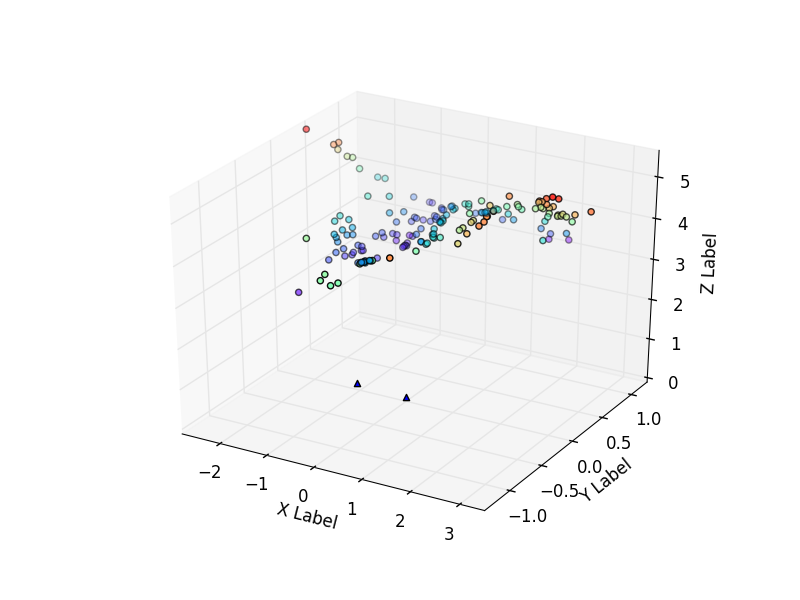
\includegraphics[width=0.4\textwidth]{house.png}
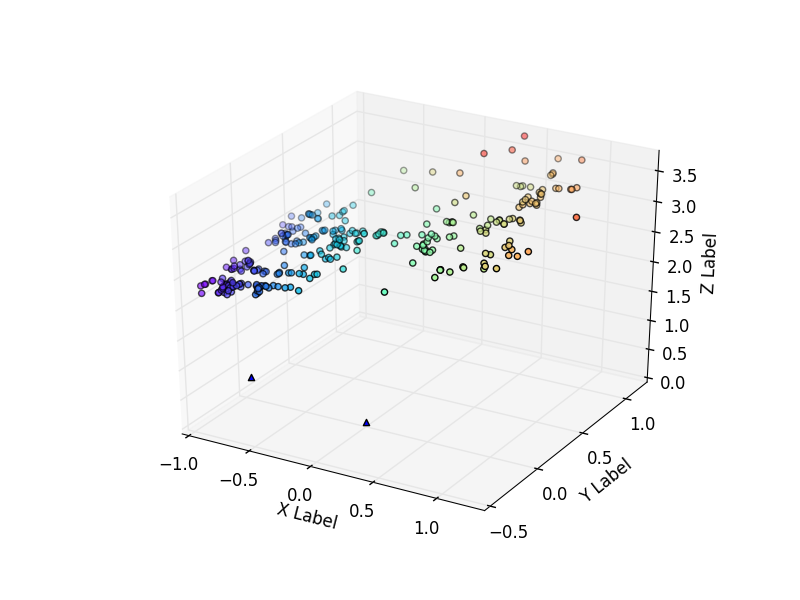
\includegraphics[width=0.4\textwidth]{library.png}
These figures show the 3D point locations for the house (left) and library (right). 

%library

\end{mdframed}

\end{document}